% !TEX root = main.tex

\section{决策树}
\subsection{信息增益}
假设当前样本$D$中第$k$类样本所占比例为$p_k$(如好瓜坏瓜二分类$M$就是$2$),则$D$的信息熵为
\[Ent(D)=-\sum_{k=1}^M p_k\log_2 p_k\]
$Ent(D)$的值越小,则$D$的纯度越高。

假设离散属性$a$有$V$个可能取值$\{a^1,a^2,\ldots,a^V\}$(如颜色属性,红蓝绿,则$a^1=R,a^2=B,a^3=G$),则产生$V$个分支结点,第$v$个结点包含取值为$a^v$的样本,记为$D^v$。
进而可以给不同分支结点赋予权值,并计算用属性$a$进行划分的信息增益(information gain)
\[Gain(D,a)=Ent(D)-\sum_{v=1}^V\frac{|D^v|}{|D|}Ent(D^v)\]
一般信息增益越大,意味着依据$a$划分所获得的纯度提升越大。
因此每次划分采用最大信息增益的属性进行划分,此即ID3(迭代二分器,Iterative Dichotomiser)决策树学习算法[Quinlan, 1986]。
\begin{figure}[H]
\centering
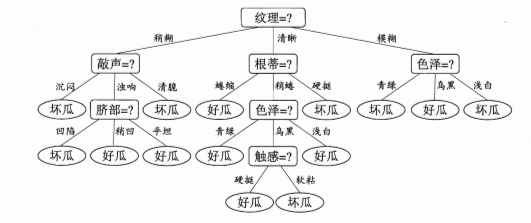
\includegraphics[width=0.6\linewidth]{fig/ID3.png}
\end{figure}

\begin{figure}[H]
\centering
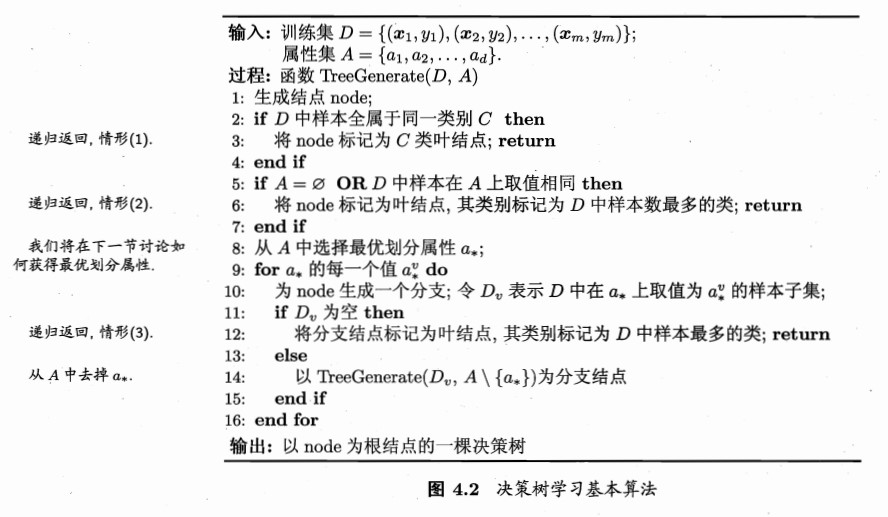
\includegraphics[width=0.8\linewidth]{fig/decision_tree.jpg}
\end{figure}

注意先前划分的指标后面可能依然会被作为划分标准,只要信息增益最大。

通过剪枝来避免过拟合
\begin{itemize}
	\item 预剪枝:对每个结点在划分前进行估计,若划分不能提升决策树泛化性能,则停止划分并将当前结点标记为叶结点,类别标记为训练样例最多的类别。
	\item 后剪枝:先完整生成一棵决策树,然后自底向上对非叶结点进行考察,若结点对应的子树替换成叶结点能够带来决策树泛化性能提升,则将该子树替换为叶结点。
\end{itemize}

类似地采用其他指标可以得到其他决策树算法:
\begin{itemize}
	\item C4.5(Classifier)算法[Quinlan ,1993]:用增益率(gain ratio)来选择最优划分属性
	\[\text{Gain\_ratio}(D,a)=\frac{\text{Gain}(D,a)}{IV(a)}\]
	其中
	\[IV(a)=-\sum_{v=1}^V\frac{|D^v|}{|D|}\log_2\frac{|D^v|}{|D|}\]
	为属性$a$的固有值(intrinsic value)。但C4.5采用启发式算法选择划分,而不是单纯基于增益率。
	\textbf{增益率准则对可取值数目较少的属性有所偏好}。
	\item CART(Classification and Regression Tree)算法[Breiman, 1984]:采用基尼指数(Gini index)
	\[\text{Gini}(D)=\sum_{k=1}^{M}\sum_{k'\ne k}p_kp_{k'}=1-\sum_{k=1}^Mp_k^2\]
	反映了从数据集$D$中随机抽取两个样本,类别标记不一致的概率。
	\[\text{Gini\_index}(D,a)=\sum_{v=1}^V\frac{|D^v|}{|D|}\text{Gini}(D^v)\]
	选择基尼指数较小的进行划分。
	CART算法包括决策树生成和决策树剪枝两个部分,回归树最小化平方误差,分类树最小化基尼指数。
\end{itemize}

理想的决策树应该是叶子结点数最少、叶子结点深度最小、叶子结点数最少且叶子结点深度最小的树。
找到这种最优的决策树是NP难题。决策树优化的目的就是要找到尽可能趋向于最优的决策树。

\subsection{连续值处理}
连续属性的离散化常用二分法,这是在C4.5算法中采用的方法。

假定连续属性$a$在$D$上出现了$n$个不同的取值,将这些值从小到大排序记为$\{a^1,a^2,\ldots,a^n\}$,基于划分点$t$可以将$D$分为子集$D_t^-$和$D_t^+$,进而可以考虑$n-1$个候选划分点集合
\[T_a=\lrb{\frac{a^i+a^{i+1}}{2}\mid 1\leq i\leq n-1}\]

\subsection{缺失值处理}
$\tilde{D}$表示$D$中在属性$a$上没有缺失值的样本子集,$\tilde{D}^v$表示$\tilde{D}$中在属性$a$上取值为$a^v$的样本子集,$\tilde{D}_k$表示$\tilde{D}$中属于第$k$类的样本子集。
为每个样本$\vx$赋予权重$w_\vx$,定义
\[\begin{aligned}
\rho &= \frac{\sum_{\vx\in\tilde{D}}w_{\vx}}{\sum_{\vx\in D}w_{\vx}}\\
\tilde{p}_k &= \frac{\sum_{\vx\in\tilde{D}_k}w_{\vx}}{\sum_{\vx\in\tilde{D}}w_{\vx}}\quad(1\leq k\leq |\mathcal{Y}|)\\
\tilde{r}_v &= \frac{\sum_{\vx\in\tilde{D}^v}w_{\vx}}{\sum_{\vx\in\tilde{D}}w_{\vx}}\quad(1\leq v\leq V)
\end{aligned}\]
分别为无缺失值样本所占的比例、无缺失样本中第$k$类所占的比例、无缺失值样本中在属性$a$上取值$a^v$的样本所占的比例。
显然有$\sum_{k=1}^{|\mathcal{Y}|}\tilde{p}_k=1$和$\sum_{v=1}^V\tilde{r}_v=1$。

可将信息增益推广为
\[\begin{aligned}
\mathrm{Gain}(D,a) &= \rho\times \mathrm{Gain}(\tilde{D},a)\\
&= \rho\times\lrp{\mathrm{Ent}\lrp{\tilde{D}}-\sum_{v=1}^V\tilde{r}_v\mathrm{Ent}\lrp{\tilde{D}^v}}
\end{aligned}\]
其中
\[\mathrm{Ent}\lrp{\tilde{D}}=-\sum_{k=1}^{|\mathcal{Y}|}\tilde{p}_k\log_2\tilde{p}_k\]

\subsection{多变量决策树}
决策树形成的分类边界有一个明显的特点,即与坐标轴平行,故学习的结果具有较好的可解释性,因为每一段划分都直接对应某个属性的取值。
但在学习任务的真实边界比较复杂时,就需要使用很多段划分才能得到比较好的近似。
\begin{figure}[H]
\centering
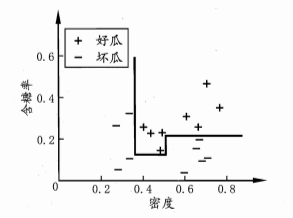
\includegraphics[width=0.4\linewidth]{fig/DT-boundary.png}
\end{figure}

如果采用线性分类器,则变成多变量决策树,可以实现更加复杂的划分。
\begin{figure}[H]
\centering
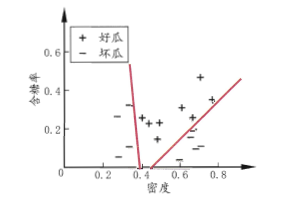
\includegraphics[width=0.4\linewidth]{fig/multivar-DT.png}
\end{figure}

决策树可能会陷入局部最优(贪心增益最高),同时分类边界表达能力弱,之后可采用随机森林的方法对性能进行提升。